\documentclass{article}
\usepackage[T1]{fontenc}

\usepackage{graphicx}
\usepackage{listings}
\begin{document}

\title{FOSS Lab Report}
\author{Gokul K\\[2\baselineskip]
Roll Number: 21\\[2\baselineskip]}
\date{02 February 2020}

\maketitle

\setcounter{section}{13}
\section{Shell Programming X}
\subsection{Aim}
Write a shell script that, given a file name as the argument will count
vowels, blank spaces, characters, number of line and symbols.

\subsection{Source Code}
\begin{verbatim}
    #! /bin/bash

    # Gokul K
    # Roll No: 21
    # 25-01-2020

    # Write a shell script that, given a file name as the argument will count
    # vowels, blank spaces, characters, number of line and symbols.

    if [[ $# -ne 1 || !(-f $1) ]]
    then
        echo "Please provide a filename"
        exit
    fi

    vc="`grep -o [aeiouAEIOU] $1 | wc -l`"
    bsc="`grep -o " " $1 | wc -l`"
    cc="`cat $1 | wc -m`"
    lc="`cat $1 | wc -l`"
    sc="`grep -o [\!\@\#\$\%\\^\&\*\(\)] $1 | wc -l`"

    printf "Number of vowels: %s\n\
    Number of blank spaces: %s\n\
    Number of characters: %s\n\
    Number of lines: %s\n\
    Number of symbols: %s\n" $vc $bsc $cc $lc $sc
\end{verbatim}

\subsection{Program Description}
grep -o command prints all matched characters specified by the pattern.
wc command with -l flag counts the number of lines in the output. Hence with a
combination of both we can find the number of matches.

\subsection{Output}
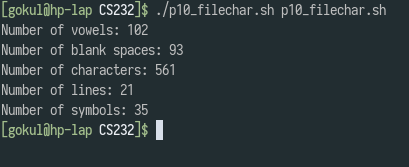
\includegraphics[width=0.9\textwidth]{img/p14.png}\newline

\subsection{Result}
The above program is run on Manjaro Linux shell. The source file itself was given
as input and the output was obtained
\end{document}